\section{Laboratorium IV}\label{sec:lab4}

\subsection{Wybrany sprzęt}\label{subsec:lab4-hw}

Enviro HAT

\subsection{Dodatkowe oprogramowanie}\label{subsec:lab4-sw}

font-roboto, bme280, ltr559, st7735, pillow, sounddevice

\subsection{Rozwiązanie}\label{subsec:lab4-sol}

Rysunek~\ref{fig:weatherlab} to~fragment instrukcji zawierający dwa~zadania.
Zadanie \emph{Z3.} wykorzystuje platformę \emph{ntfy.sh} do~wysłania powiadomienia w~momencie przykrycia czujnika
zbliżeniowego na~płytce, informacje zawarte w~tej wiadomości przedstawia rysunek~\ref{fig:weatherntfy}.
W~zadaniu \emph{Z4.} student wykorzystuje poprzednio uzupełnione funkcje do~złożenia pętli głównej obsługującej program
założony w~temacie laboratorium.

\begin{figure}[H]
  \centering
  \includegraphics[width=0.9\linewidth]{media/weather_lab}
  \caption{Fragment instrukcji IV}
  \label{fig:weatherlab}
\end{figure}

\begin{figure}[H]
  \centering
  \includegraphics[width=0.9\linewidth]{media/weather_ntfy}
  \caption{Powiadomienie platformy \emph{ntfy}}
  \label{fig:weatherntfy}
\end{figure}

Rysunek~\ref{fig:weather} przedstawia rozwiązanie zadania.
Program wyświetla kolejno zbierane dane wraz~z~wykresami wcześniejszych wartości.

\begin{figure}[H]
  \centering
  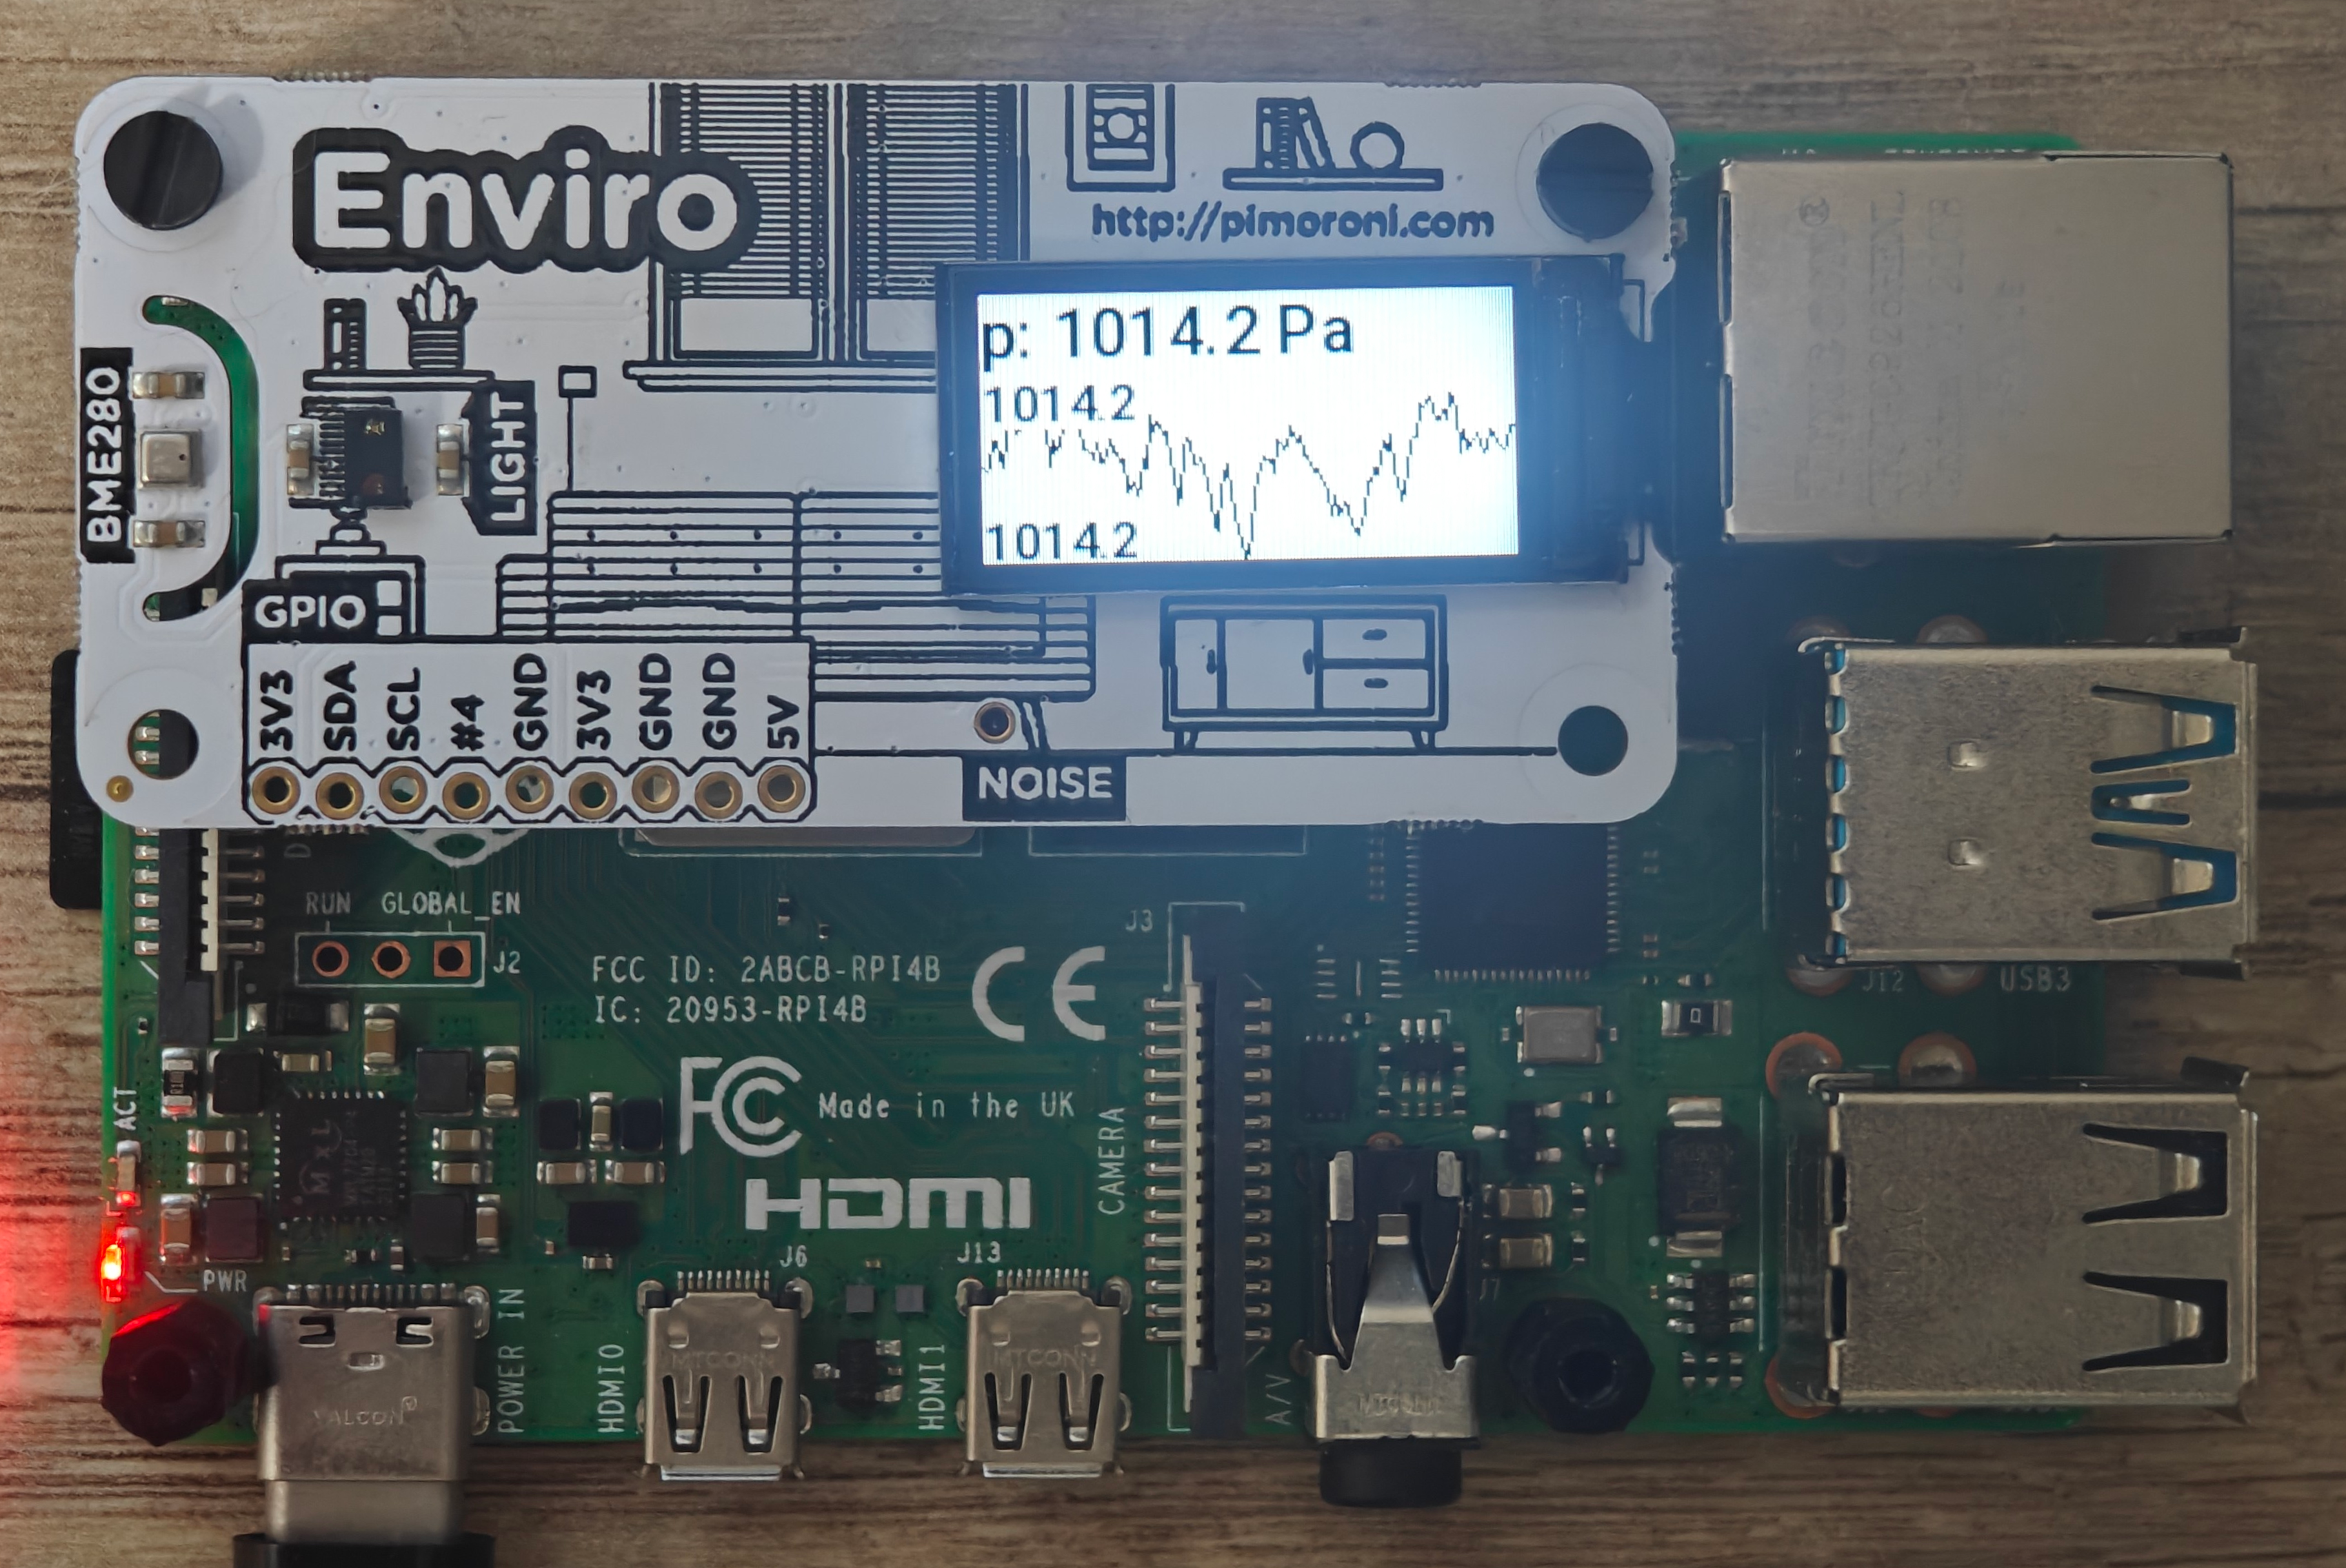
\includegraphics[width=0.6\linewidth]{media/weather}
  \caption{Uruchomiony program czwartego laboratorium}
  \label{fig:weather}
\end{figure}
